

%-------------------------------------------------------------------------------
% Dokumenten Klasse
\documentclass[
	final,
	a4paper,
	oneside,
	parskip=full,
	headings=standardclasses,
	headings=big,
	pointednumbers
]{scrartcl}

%-------------------------------------------------------------------------------
% Packete nutzen
\usepackage[T1]{fontenc}
\usepackage[utf8]{inputenc}
\usepackage[left=15mm,right=20mm,top=17mm,bottom=17mm,footskip=0.7cm]{geometry}
\usepackage{amsmath}
\usepackage{amssymb}
\usepackage{mathtools}
\usepackage{mathtools}
\usepackage{bm}

%-------------------------------------------------------------------------------
% Andere Schriftart
\usepackage{lmodern}

%-------------------------------------------------------------------------------
% xcolor
\usepackage[svgnames,table]{xcolor}

%-------------------------------------------------------------------------------
% scrlayer-scrpage
\usepackage{scrlayer-scrpage}
\pagestyle{scrheadings}
\clearpairofpagestyles

\cfoot{\pagemark}

%-------------------------------------------------------------------------------
% array
\usepackage{array}
\newcolumntype{A}[1]{>{\raggedright\let\newline\\\arraybackslash\hspace{0pt}}p{#1}}
\newcolumntype{B}[1]{>{\centering\let\newline\\\arraybackslash\hspace{0pt}}p{#1}}
\newcolumntype{C}[1]{>{\raggedleft\let\newline\\\arraybackslash\hspace{0pt}}p{#1}}

\newcolumntype{D}[1]{>{\raggedright\let\newline\\\arraybackslash\hspace{0pt}}m{#1}}
\newcolumntype{E}[1]{>{\centering\let\newline\\\arraybackslash\hspace{0pt}}m{#1}}
\newcolumntype{F}[1]{>{\raggedleft\let\newline\\\arraybackslash\hspace{0pt}}m{#1}}

\newcolumntype{G}[1]{>{\raggedright\let\newline\\\arraybackslash\hspace{0pt}}b{#1}}
\newcolumntype{H}[1]{>{\centering\let\newline\\\arraybackslash\hspace{0pt}}b{#1}}
\newcolumntype{I}[1]{>{\raggedleft\let\newline\\\arraybackslash\hspace{0pt}}b{#1}}


%-------------------------------------------------------------------------------
% tabularx
\usepackage{tabularx}
\usepackage{ltablex}
\usepackage{makecell}

%-------------------------------------------------------------------------------
% TikZ
\usepackage{tikz}
\usetikzlibrary{shapes, positioning, arrows, decorations, calc, fit, intersections}

%-------------------------------------------------------------------------------
% Listings
\usepackage{listings}
\newcommand{\listingMatlab}[2][]{
	\lstset{
		language=Matlab,
		breaklines=true,
		numbers=left,
		numberstyle=\tiny,
		numbersep=5pt,
		captionpos=b,
		basicstyle=\footnotesize\ttfamily,
		stringstyle=\color{magenta},
		identifierstyle=\color{black},
		keywordstyle=\color{blue}, 
		commentstyle=\color{DarkGreen}
	}
	\lstinputlisting[caption={\texttt{\detokenize{#2}}},#1]{#2}
}
\lstnewenvironment{algorithm}[1][] %defines the algorithm listing environment
{
    \lstset{ %this is the stype
        mathescape=true,
        frame=tB,
        numbers=left, 
        numberstyle=\tiny,
        basicstyle=\scriptsize, 
        keywordstyle=\color{black}\bfseries,
        keywords={,input, output, return, datatype, function, in, if, else, foreach, while, begin, end, } 
        numbers=left,
        xleftmargin=.04\textwidth
    }
}
{}


%-------------------------------------------------------------------------------

\RedeclareSectionCommand[
  afterindent=false,
  beforeskip=0.8\baselineskip,
  afterskip=0.4\baselineskip]{section}
\RedeclareSectionCommand[
  afterindent=false,
  beforeskip=0.8\baselineskip,
  afterskip=0.4\baselineskip]{subsection}

%-------------------------------------------------------------------------------
% 

\newcommand{\colouredcircle}{%
    \tikz{
        \useasboundingbox (-0.2em,-0.32em) rectangle(0.2em,0.32em);
        \draw[line width=0.03em] (0,0) circle(0.10em);
    }}



%-------------------------------------------------------------------------------
% enumitem
\usepackage{enumitem}
\newlist{tabenum}{enumerate}{3}
\setlist[tabenum,1]{
    leftmargin=*,
    label=\protect\colouredcircle,
    topsep=0ex,
    partopsep=0ex,
    noitemsep
}
\setlist[tabenum,2]{
    leftmargin=*,
    label=\protect\colouredcircle,
    topsep=0ex,
    partopsep=0ex,
    noitemsep
}
\setlist[tabenum,3]{
    leftmargin=*,
    label=\protect\colouredcircle,
    topsep=0ex,
    partopsep=0ex,
    noitemsep
}

\newcommand{\f}[2]{\frac{#1}{#2}}
\newcommand{\fs}[2]{{\tfrac{#1}{#2}}}

% kl = ()
\newcommand{\kl}[1]{{\left( #1 \right)}}

% kq = {}
\newcommand{\kq}[1]{{\left\{ #1 \right\}}}

% ks = []
\newcommand{\ks}[1]{{\left[ #1 \right]}}

% 
\newcommand{\abs}[1]{{\vert #1 \vert}}


\newcommand{\txb}[1]{{\color{blue}#1}}
\newcommand{\txr}[1]{{\color{red}#1}}
\newcommand{\txo}[1]{{\color{orange}#1}}
\newcommand{\txgr}[1]{{\color{grey}#1}}
\newcommand{\tb}[1]{\textbf{#1}}
\newcommand{\ti}[1]{\textit{#1}}

\newcommand{\tc}[1]{\multicolumn{1}{r|}{#1}}

%-------------------------------------------------------------------------------
% 
\usepackage{xparse}
% 1: Subscription  (default: '')
% 2: Funktion Name (default: 'f')
% 3: Argument      (default: 'x')
% \fx         = f(x)
% \fx[1]      = f_1(x)
% \fx[][u]    = u(x)
% \fx[][u][x] = u(x)
% \fx[][f][u] = f(u)
\NewDocumentCommand{\fx}{ O{} O{f} O{x} }{{#2_{#1}{\left( #3 \right)}}}
\NewDocumentCommand{\dfx}{ O{} O{f} O{x} }{{#2'_{#1}{\left( #3 \right)}}}
\NewDocumentCommand{\dx}{ O{} }{{\Delta x^{#1}}}
\NewDocumentCommand{\dy}{ O{} }{{\Delta y^{#1}}}
\NewDocumentCommand{\dt}{ O{} }{{\Delta t^{#1}}}
\NewDocumentCommand{\du}{ O{} }{{\Delta u^{#1}}}
\NewDocumentCommand{\px}{ O{} }{{\partial x^{#1}}}
\NewDocumentCommand{\py}{ O{} }{{\partial y^{#1}}}
\NewDocumentCommand{\pt}{ O{} }{{\partial t^{#1}}}
\NewDocumentCommand{\pu}{ O{} }{{\partial u^{#1}}}
\NewDocumentCommand{\p}{ O{} }{{\partial^{#1}}}
\NewDocumentCommand{\re}{ O{} }{{\mathbb{R}^{#1}}}

\NewDocumentCommand{\xyz}{ O{x} O{y} O{z} }{#1 #2 #3}
% 1: Value
% 2: Key
% 3: Background Color
\NewDocumentCommand{\tfill}{ O{} O{} O{blue!20} }{%
    \tikz[baseline, every node/.style={inner sep=3pt,outer sep=0pt,minimum width=3mm,minimum height=4mm}]{
        \node[fill=#3,anchor=base] (#2) {#1};
    }
}
\NewDocumentCommand{\tfillc}{ O{} O{} }{%
    \tikz[baseline, every node/.style={inner sep=2pt,outer sep=0pt}]{
        \node[fill=#2,anchor=base] {#1};
    }
}

\NewDocumentCommand{\tdrawc}{ O{} O{} }{%
    \tikz[baseline, every node/.style={inner sep=2pt,outer sep=0pt}]{
        \node[rectangle,draw=#2,anchor=base] {#1};
    }
}

\NewDocumentCommand{\tcrossc}{ O{} O{} }{%
    \tikz[baseline, every node/.style={inner sep=0pt,outer sep=0pt}]{
        \node[draw=#2,anchor=base,cross out,line width=1pt] {#1};
    }
}

\newcommand{\tfillb}[1]{\tfillc[#1][blue!20]}
\newcommand{\tfillo}[1]{\tfillc[#1][orange!40]}
\newcommand{\tfillg}[1]{\tfillc[#1][Green!20]}
\newcommand{\tfilly}[1]{\tfillc[#1][yellow!40]}
\newcommand{\tfillr}[1]{\tfillc[#1][red!20]}
\newcommand{\tfillv}[1]{\tfillc[#1][Violet!20]}
\newcommand{\tfillt}[1]{\tfillc[#1][Turquoise!20]}
\newcommand{\tfillgr}[1]{\tfillc[#1][Gray!20]}


\newcommand{\tdrawb}[1]{\tdrawc[#1][blue!40]}
\newcommand{\tdrawo}[1]{\tdrawc[#1][orange!60]}
\newcommand{\tdrawg}[1]{\tdrawc[#1][Green!40]}
\newcommand{\tdrawy}[1]{\tdrawc[#1][yellow!60]}
\newcommand{\tdrawr}[1]{\tdrawc[#1][red!40]}
\newcommand{\tdrawv}[1]{\tdrawc[#1][Violet!40]}
\newcommand{\tdrawt}[1]{\tdrawc[#1][Turquoise!40]}
\newcommand{\tdrawgr}[1]{\tdrawc[#1][Gray!40]}
\newcommand{\tdrawk}[1]{\tdrawc[#1][black]}


\newcommand{\tcrossr}[1]{\tcrossc[#1][red]}
\newcommand{\tcrossg}[1]{\tcrossc[#1][green]}
\newcommand{\tcrossb}[1]{\tcrossc[#1][blue]}

\begin{document}
    \section*{StatQuest: ROC and AUC}

    This StatQuest builds on the \tb{Confusion Matrix} and the \tb{Sensitifity and Specificity}
    StatQuests. So if you're not already down with those, check out the Quests.

    Also, the examples I give in this StatQuest is based on Logistic Regression, so, even though
    \tb{ROC} and \tb{AUC} apply to more than just Logistic Regression, make sure you
    understand those basics.

    Let's start with some data.

    \begin{center}
        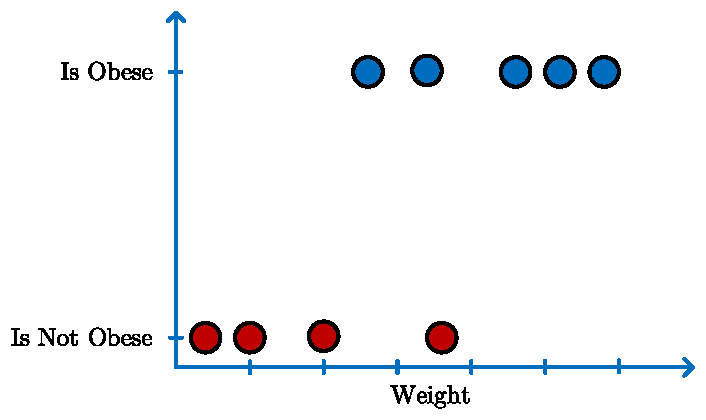
\includegraphics[height=5cm]{StatQuest_ROC_and_AUC_Obese.pdf}
    \end{center}

    The y-axis has two categories: ``obese'' and ``not obese''.
    The \txb{blue dots} represent obese mice and the \txr{red dots} represent mice that are not obese.

    Along the x-axis, we have \tb{weight}.

    The last red dot is a mouse that is not obese,
    even though it weighs a lot. It must be ``Mighty Mouse'' and just full of muscles.

    The first blue dot is a mouse that doesn't weigh that much, but it is still considered
    obese for its size.

    Now let's fit a Logistic Regression curve to the data.

    \begin{center}
        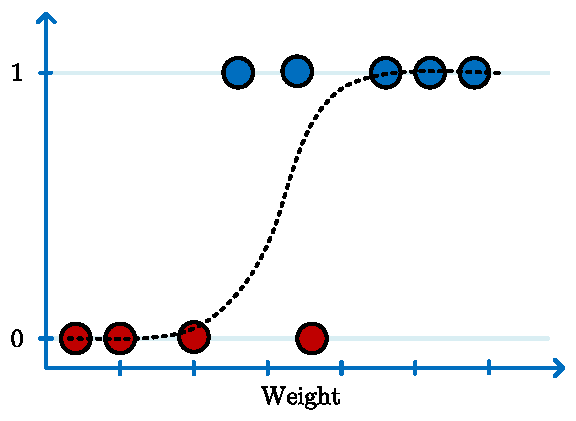
\includegraphics[height=5cm]{StatQuest_ROC_and_AUC_Obese_Probability.pdf}
    \end{center}

    When we're doing Logistic Regression, the y-axis is converted to the probability
    that a mouse is obese. Now, let's just look at the curve.

    \newpage

    If someone told us that they had a heavy mouse that weighs this much, then the curve would
    tell us that there is a \tb{high} probability that the mouse is obese.

    \begin{center}
        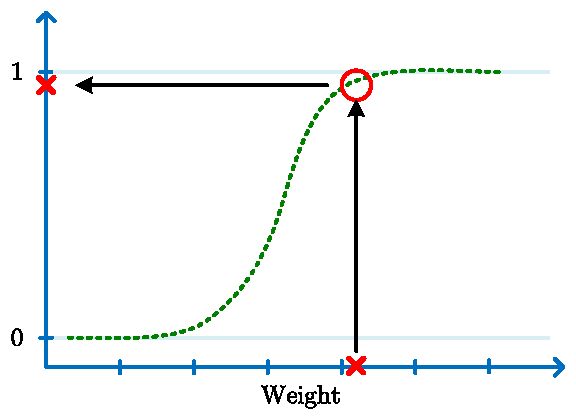
\includegraphics[height=5cm]{StatQuest_ROC_and_AUC_Obese_HighProbability.pdf}
    \end{center}

    If someone told us that they had a light mouse that weighs this much, then the curve
    would tell us that there is a \tb{low} probability that the mouse is obese.

    \begin{center}
        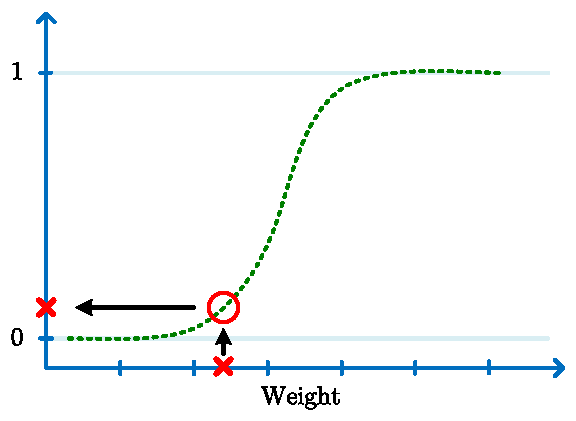
\includegraphics[height=5cm]{StatQuest_ROC_and_AUC_Obese_LowProbability.pdf}
    \end{center}

    So this Logistic Regression tells us the \tb{probability} tat a mouse is
    obese based on its weight. However, if we want to \tb{classify} the mice as
    \txb{obese} or \txr{not obese}, then we need a way to turn probabilities
    into classifications.

    One way to classify mice is to set a threshold at $\bm{0.5}$ and
    classify all mice with a probability of being obese $\bm{> 0.5}$ as \txb{obese}
    and classify all mice with a probability of being obese $\bm{\leq 0.5}$ as \txr{not obese}.

    \begin{center}
        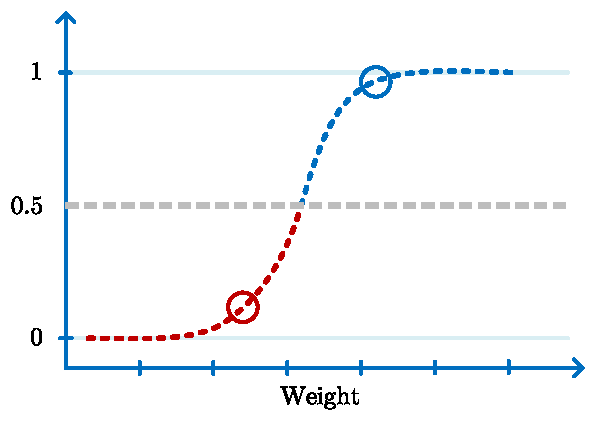
\includegraphics[height=5cm]{StatQuest_ROC_and_AUC_Obese_Threshold.pdf}
    \end{center}



    

\end{document}